\documentclass[border=10pt]{standalone}

\usepackage{tikz}
\usepackage{tikzsymbols}
\usetikzlibrary{calc,patterns,shapes.geometric}

\def\centerarc[#1](#2)(#3:#4:#5){\draw[#1] ($(#2)+({#5*cos(#3)},{#5*sin(#3)})$) arc (#3:#4:#5);}

\begin{document}
	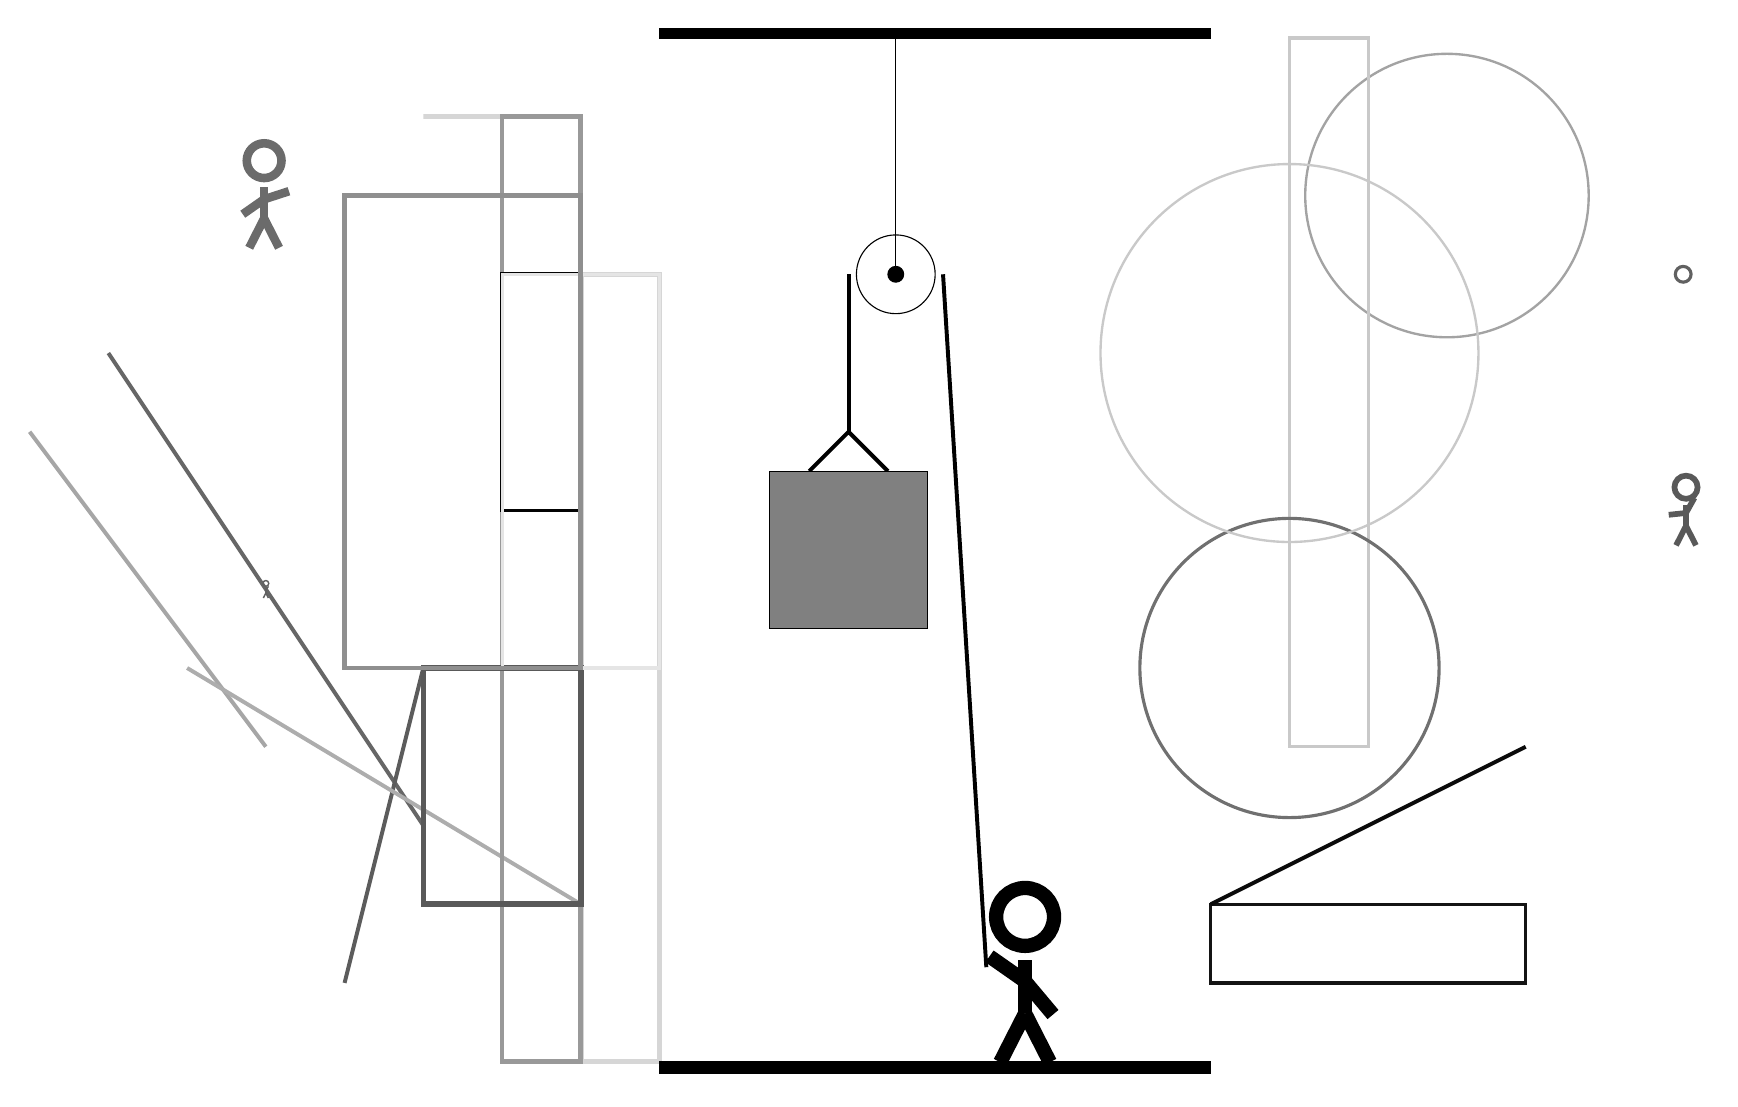
\begin{tikzpicture}
		%%%%% START %%%%%
		
		\draw[fill=black] (-2, 10) rectangle (5, 10.125);
		
		\draw (1, 7) circle (0.5);
		\draw[fill=black] (1, 7) circle (0.1);
		\draw (1, 10) -- (1, 7);
		
		\draw[line width=0.3mm, color=black!77] (-4, -1) rectangle (-4, 7);
		
		\draw[line width=0.4mm, color=black!92] (5, -2) rectangle (9, -1);
		\draw [line width=0.3mm, color=black!36](8, 8) circle (1.8);
		\draw[line width=0.4mm, color=black!21] (6, 1) rectangle (7, 10);
		\draw[line width=0.5mm, color=black!60](-5, 0) -- (-9, 6);
		\draw[line width=0.6mm, color=black!16] (-3, 9) rectangle (-5, 9);
		
		\draw[line width=0.5mm, color=black!64](-6, -2) -- (-5, 2);
		
		\draw[line width=0.5mm, color=black!96](9, 1) -- (5, -1);
		\draw[line width=0.5mm, color=black!35](-7, 1) -- (-10, 5);
		\draw[line width=0.7mm, color=black!16] (-3, 7) rectangle (-2, -3);
		
		\node[line width=0.6mm, color=black!65] at (11, 4) {\Strichmaxerl[4][6][61]};
		
		\node[line width=0.3mm, color=black!62] at (-7, 3) {\Strichmaxerl[1][90][53]};
		\draw[line width=0.5mm, color=black!32](-3, -1) -- (-8, 2);
		
		\draw[line width=0.6mm, color=black!40] (-3, 9) rectangle (-4, -3);
		\node[line width=0.6mm, color=black!58] at (-7, 8) {\Strichmaxerl[6][35][18]};
		\draw [line width=0.4mm, color=black!56](6, 2) circle (1.9);
		
		\draw [line width=0.4mm, color=black!62](11, 7) circle (0.1);
		\draw[line width=0.5mm, color=black!99] (-4, 7) rectangle (-3, 4);
		\draw[line width=0.7mm, color=black!65] (-3, 2) rectangle (-5, -1);
		
		\draw[line width=0.4mm, color=black!10] (-2, 7) rectangle (-4, 2);
		\draw[line width=0.6mm, color=black!44] (-3, 8) rectangle (-6, 2);
		
		\draw [line width=0.3mm, color=black!21](6, 6) circle (2.4);
		
		
		\draw[line width=0.5mm] (-0.1, 4.5) -- (0.4, 5.0) -- (0.9, 4.5);
		\draw[fill=black!50] (-0.6, 4.5) rectangle (1.4, 2.5);
		
		\draw[line width=0.5mm] (0.4, 7) -- (0.4, 5.0);
		\centerarc[line width=0.5mm](1, 7)(0:180:0.6);
		\draw[line width=0.5mm](1.6, 7) -- (2.15, -1.8);
		
		\node at (2.6, -1.9) {\Strichmaxerl[10][-35][-50]};
		
		\draw[fill=black] (-2, -3) rectangle (5, -3.15);
		
		%%%%% END %%%%%
	\end{tikzpicture}
\end{document}